\documentclass{article}
\usepackage{graphicx} % Required for inserting images
\usepackage{float}
\usepackage{hyperref}
\hypersetup{
    colorlinks=true,
    linkcolor=blue,
    filecolor=magenta,      
    urlcolor=cyan,
    pdftitle={Overleaf Example},
    pdfpagemode=FullScreen,
    }

\urlstyle{same}
\title{HTML GAME : MINESWEEPER CRICKET}
\author{Nandan Manjunath Immadisetty}
\date{}
\begin{document}

\maketitle

\section{About Game}
This game is a hybrid of minesweeper and cricket game. In this game, you have to select random boxes, and you will be awarded that score  and it will be added to your total score. 11 fielders will be randomly placed in the total grid, and selecting a box with a fielder costs you a life(wicket). Chase the target displayed before all your lives(wickets) are gone to win the match.
The Game is similar to actual cricket game rules and it is a luck based game.

\section{Detailed explanation of each part of the game}
\subsection{Title}
Displays the name of the game i.e. MINESWEEPER CRICKET
\subsection{MAIN BODY}
This is where the game is played. Before starting the game it shows an image(logo of the game) and after starting the game it contains a big box that has small square boxes whose number depends on the grid size. Selecting each box gives you runs which add to your score or takes a life if you selected a box containing fielder\\
\textbf{Score:} The score one can get on each click is between 0 and 6 (both included). This number is generated randomly using random function and making it an integer using the score function\\
\textbf{Fielders:}Eleven fielders are randomly placed.
After the game is over it displays a photo showing whether you won or lost.
\subsection{Scorecard}
It shows the score and number of balls played by each player in your team before getting out.
Each player's name is player0,player1 $\cdots$ and the score hit by them is displayed adjacent to their name.\\
The number of balls played by each player is displayed beside score.\\
Even the strikerate rate of each player is also displayed beside number of balls played.
The scorecard changes dynamically after every click till you win or lose the game
\subsection{Man of the match}
If the player wins the game the batsman who hits the highest score will be awarded man of the match by displaying the name of the batsman who won the man of the match below the scorecard.\\
If the player loses, there will be no man of the match.
\subsection{Striker of the match}
If the player wins the game, the batsman who has the highest strikerate will be awarded man of the match by displaying the name of the batsman who won the man of the match below man of the match.
\subsection{GAMESTART}
There are some options that you have to select before the start of the game.
\subsubsection{players}
Here we have to select how many wickets match you want to play. It has four options.
\begin{itemize}
    \item 1 wicket match. you have only one life.
    \item 2 wicket match. you have two lives.
    \item 5 wicket match. you have five lives. 
    \item 6 wicket match. you have six lives. 
\end{itemize}
you will have more fun if you select a five-wicket or six-wicket match.
\subsubsection{Difficulty}
There are four levels, and accordingly grid size will change.
\begin{itemize}
    \item \textbf{Easy} in this the grid size will be $9\times9$
    \item \textbf{Medium} in this the grid size will be $8\times8$
    \item \textbf{Difficult} in this the grid size will be $7\times7$
    \item \textbf{Asian} in this the grid size will be $6\times6$
\end{itemize}
\subsection{Gamestart button}
On clicking this button game begins\\
It calls the function startGame();
\subsection{Score,Overs,RunRate, Wickets, Six-O-Meter}
After clicking start game this box shows the team's total score, the total number of overs played,RunRate of the team,how many lives(wickets) you have lost till now and number of sixes hit till now. It changes dynamically after every ball.
\subsection{Target}
A function target is called which displays the target after starting of the game and in order to win the game we have to chase the target(our score should be $>=$ target mentioned) before all our wickets(lives) are lost
The target is generated randomly based on based on number of lives(wickets) you are having.
\begin{itemize}
    \item 1 wicket match. The target is between 1 and 40.
    \item 2 wicket match. The target is between 20 and 60.
    \item 5 wicket match. The target is between 40 and 100. 
    \item 6 wicket match. The target is between 60 and 120 
\end{itemize}
\subsection{Lost win Tag}
This appears after the game is over.\\
If you win the match it says by how many wickets you have won the match.\\
If you lose the match, it says by how many runs you have lost the match.\\
A button appears beside it, and on clicking you can come back to the start of the page where you can start a new game.
\section{List of functions used- One line description of each function}
\begin{enumerate}
    \item \textbf{startGame()} Runs on clicking start game button.Changes the page completely by removing some elements, displaying other elements which were not visible before and modifying the main body with a background of cricket ground with different cells in it.
    \item \textbf{placeFielders(num\_of\_rows)} places eleven fielders randomly in the grid by assigning row and column numbers where the fielder has to be placed. It takes an input of num\_of\_rows from the Difficulty level.It is called by startGame function.
    \item \textbf{createTable(num\_of\_rows)} This creates the grid and gives dynamic properties to it. It is called by the startGame function.
    \item \textbf{scorecardcreate(wickets)} It adds the name of the new player in the scorecard after a player is out.
    \item \textbf{generatetarget(wickets)} Generates target.
    \item \textbf{usescore()} It takes the input of the total score from the webpage and it is used by other functions.
    \item \textbf{handleCellClick(cell, i, j)} This is the main function which controls many things and it is called whenever a cell is clicked.
    It does
    \begin{itemize}
        \item If game is over on clicking any cell it does nothing.
        \item It takes care that if you click the cell twice it will consider only the first time
        \item If a wicket falls it calls all the required functions.
        \item It calls all function which need to be run after every click.
        
    \end{itemize}
    \item updateScore(score) updates score after every click. Called by handleCellClick function
    \item \textbf{checkWin()} checks whether the target is chased or not and accordingly changes the layout of the webpage.
    \item \textbf{gameOver()} Is called when you lost the match.
    \item \textbf{manofthematch()} Is called after winning the match.Shows which batsman hit the highest score and awards him man of the match by displaying his name. 
    \item \textbf{sixmeter} Updates the number of sixes hit till now after every six
    \item \textbf{Overs} Updates the number of overs happened till now.
    \item \textbf{SRgenerator} Generates strikerate of each player after every ball
    \item \textbf{strikerofthematch} If team wins, displays the team member name who has the highest strike rate and awards him striker of the match
    \item \textbf{generaterunrate} Generates runrate after every ball.
\end{enumerate}
I used a lot of cricket terms here assuming that you know the rules of cricket.
\section{Customization}
Listing them once again.
\begin{itemize}
    \item \textbf{Variable GridSize} for options are given which can be selected based on difficulty.
    \item \textbf{Can be played as multiplayer}
    As you can select a match with more number of wickets each wicket can be played by one person but all players must play in same computer.
    \item \textbf{ScoreCard} showing a detailed scorecard displaying score of each batsmen and how many balls he had played giving the player the real game feel.
    \item \textbf{Variable runs} On click you are awarded a score between 0 and 6.
    \item \textbf{number of wickets} Added a feature where you can select how many wickets match you want to play.
    \item \textbf{Target} to be chased down to decide you have won or lost.
    \item \textbf{Man of the match}
    \item \textbf{Striker of the match} basically distributing awards to each player
    \item displaying the Strike rate of each player
    \item displaying number of sixes hit till now using using Six-O-meter
    \item displaying Overs, RunRate, Wickets, score
    \item shows a duck symbol adjacent to player score if player is out without hitting runs 
    \item displaying a bat symbol adjacent to player name if the batsmen is still not out
    \item Made as many changes as possible by giving it real cricket game feel.
    \item \textbf{Visual Appeal} made it beautiful by adding background image of stadium and playing ground.showing the score on the cell after click and showing an image of being bowled if a fielder is placed in that cell.Also added beautiful images displaying whether you won or lost at the end.
    \item Added rules on starting page so that people who don't know about the game can understand.
\end{itemize}
Made this game similar to real cricket game. I myself loved playing the game which I created and liked it and hope you will also like it.
\section{Images}
\begin{figure}[H]
    \centering
    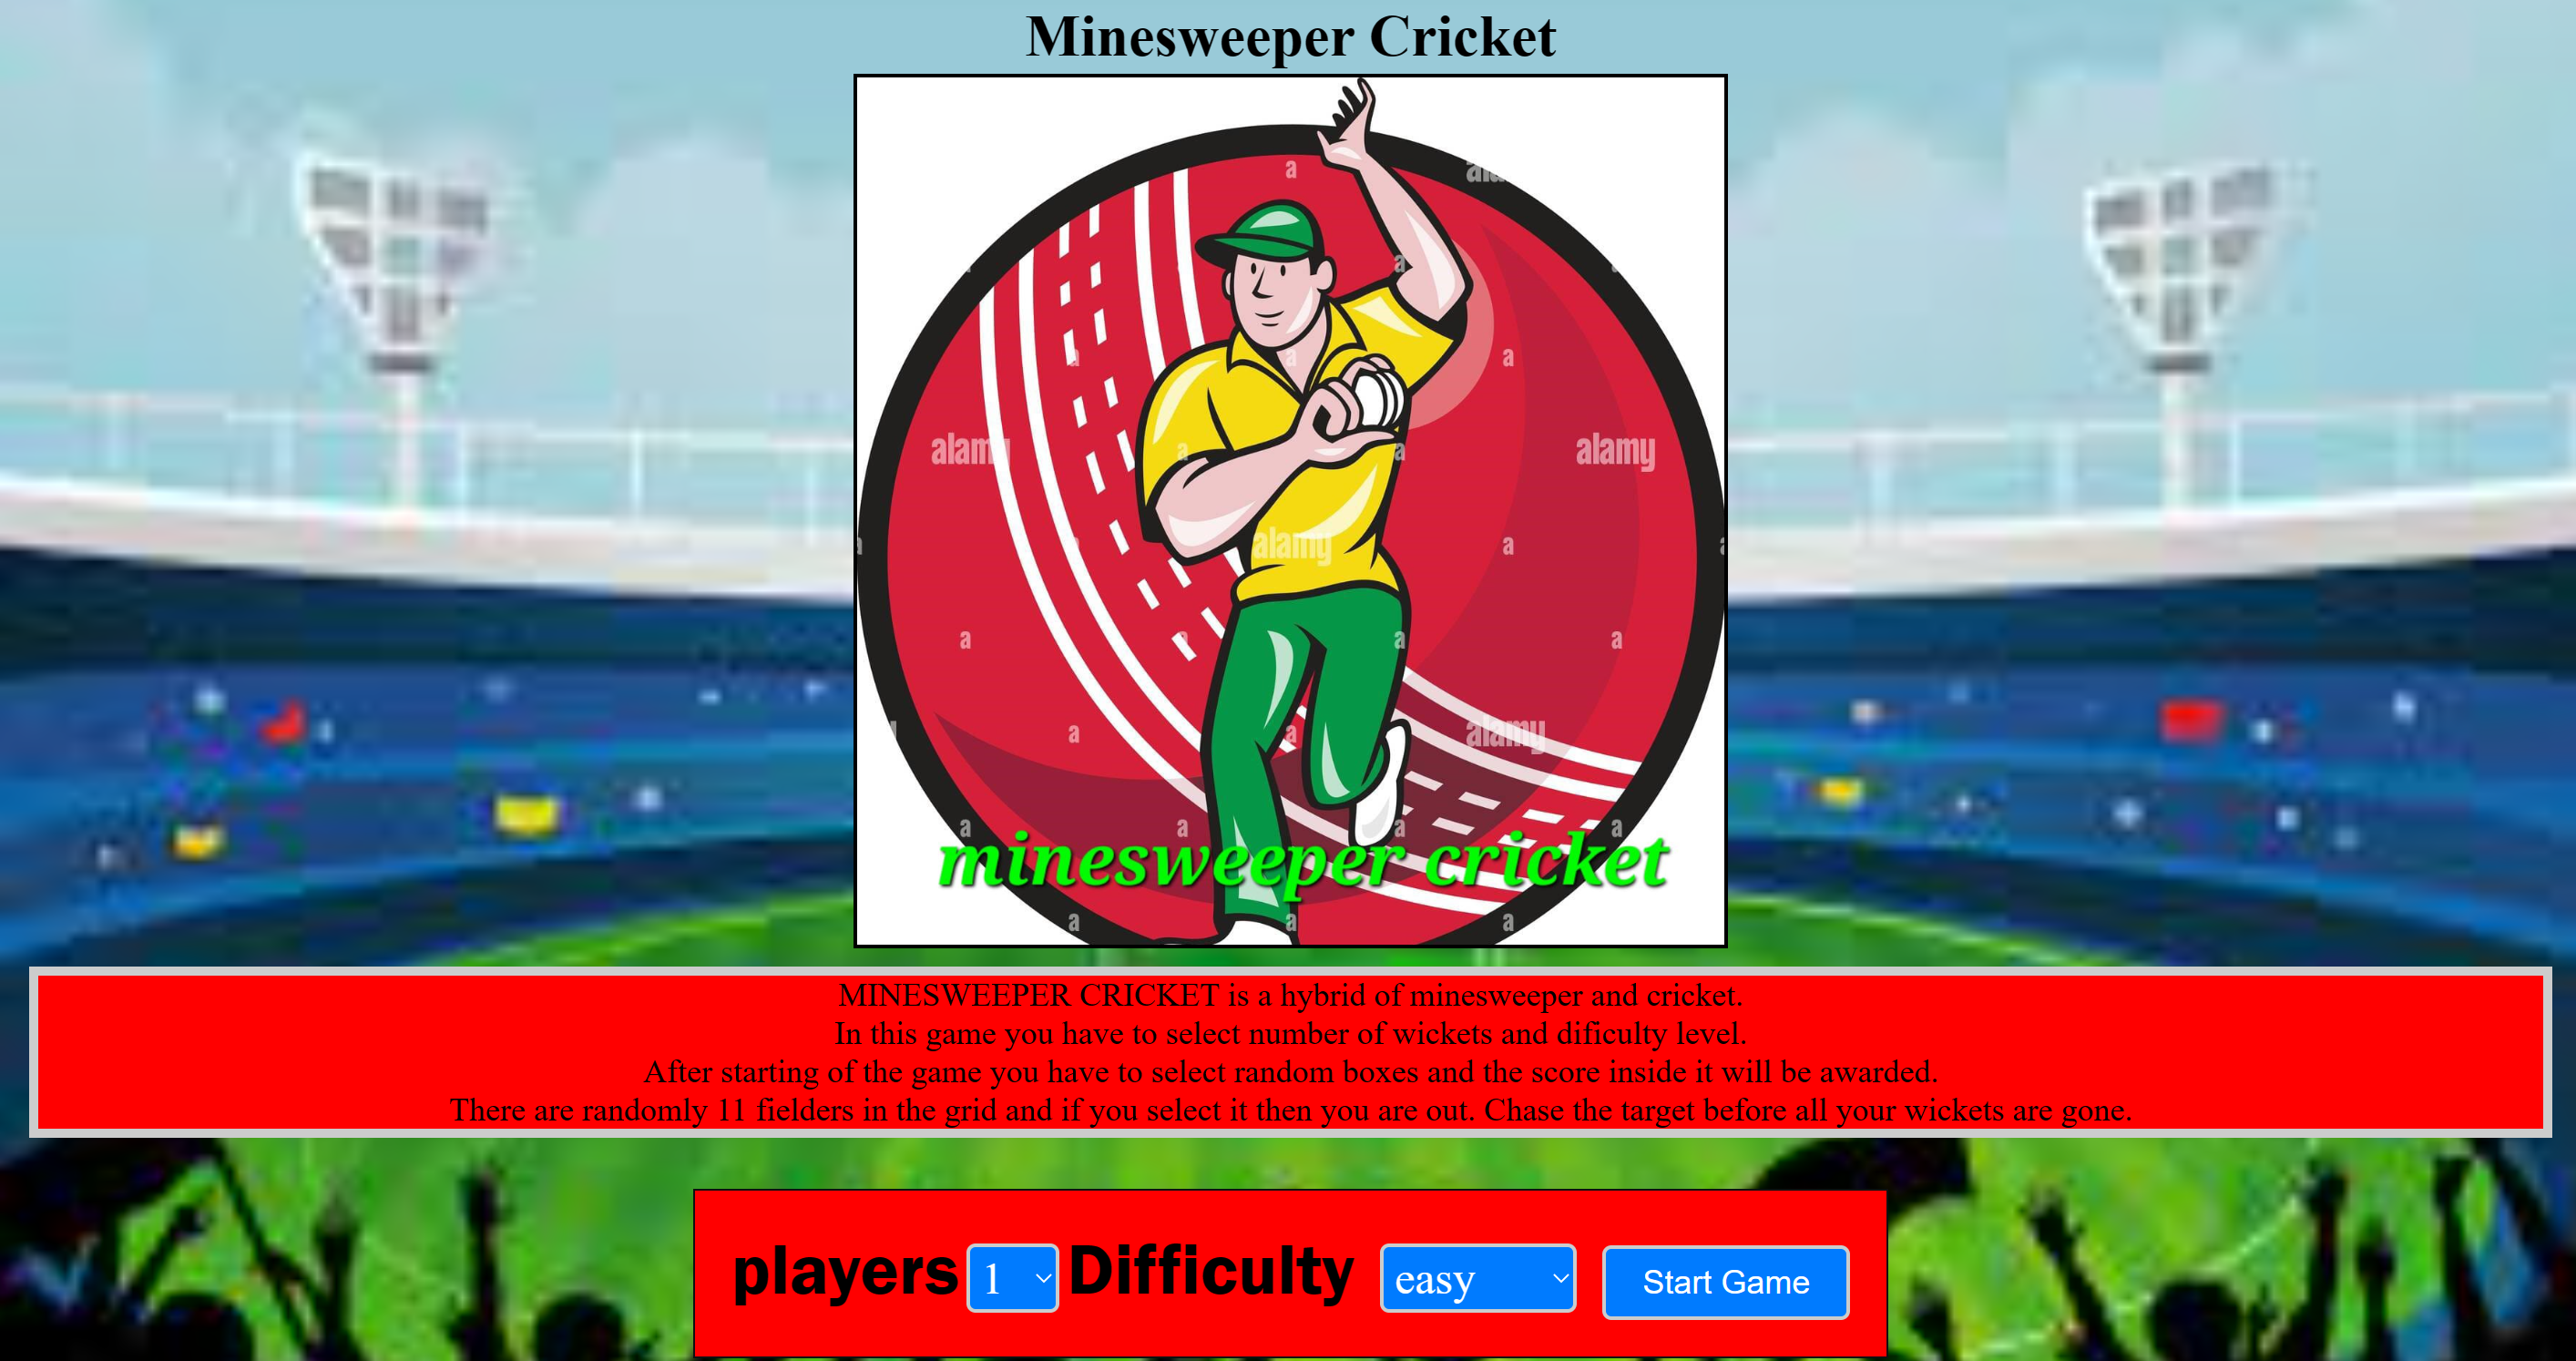
\includegraphics[width=1\textwidth]{homepage}
    \caption{Before starting of game}
    \label{fig:enter-label}
\end{figure}
\begin{figure}[H]
    \centering
    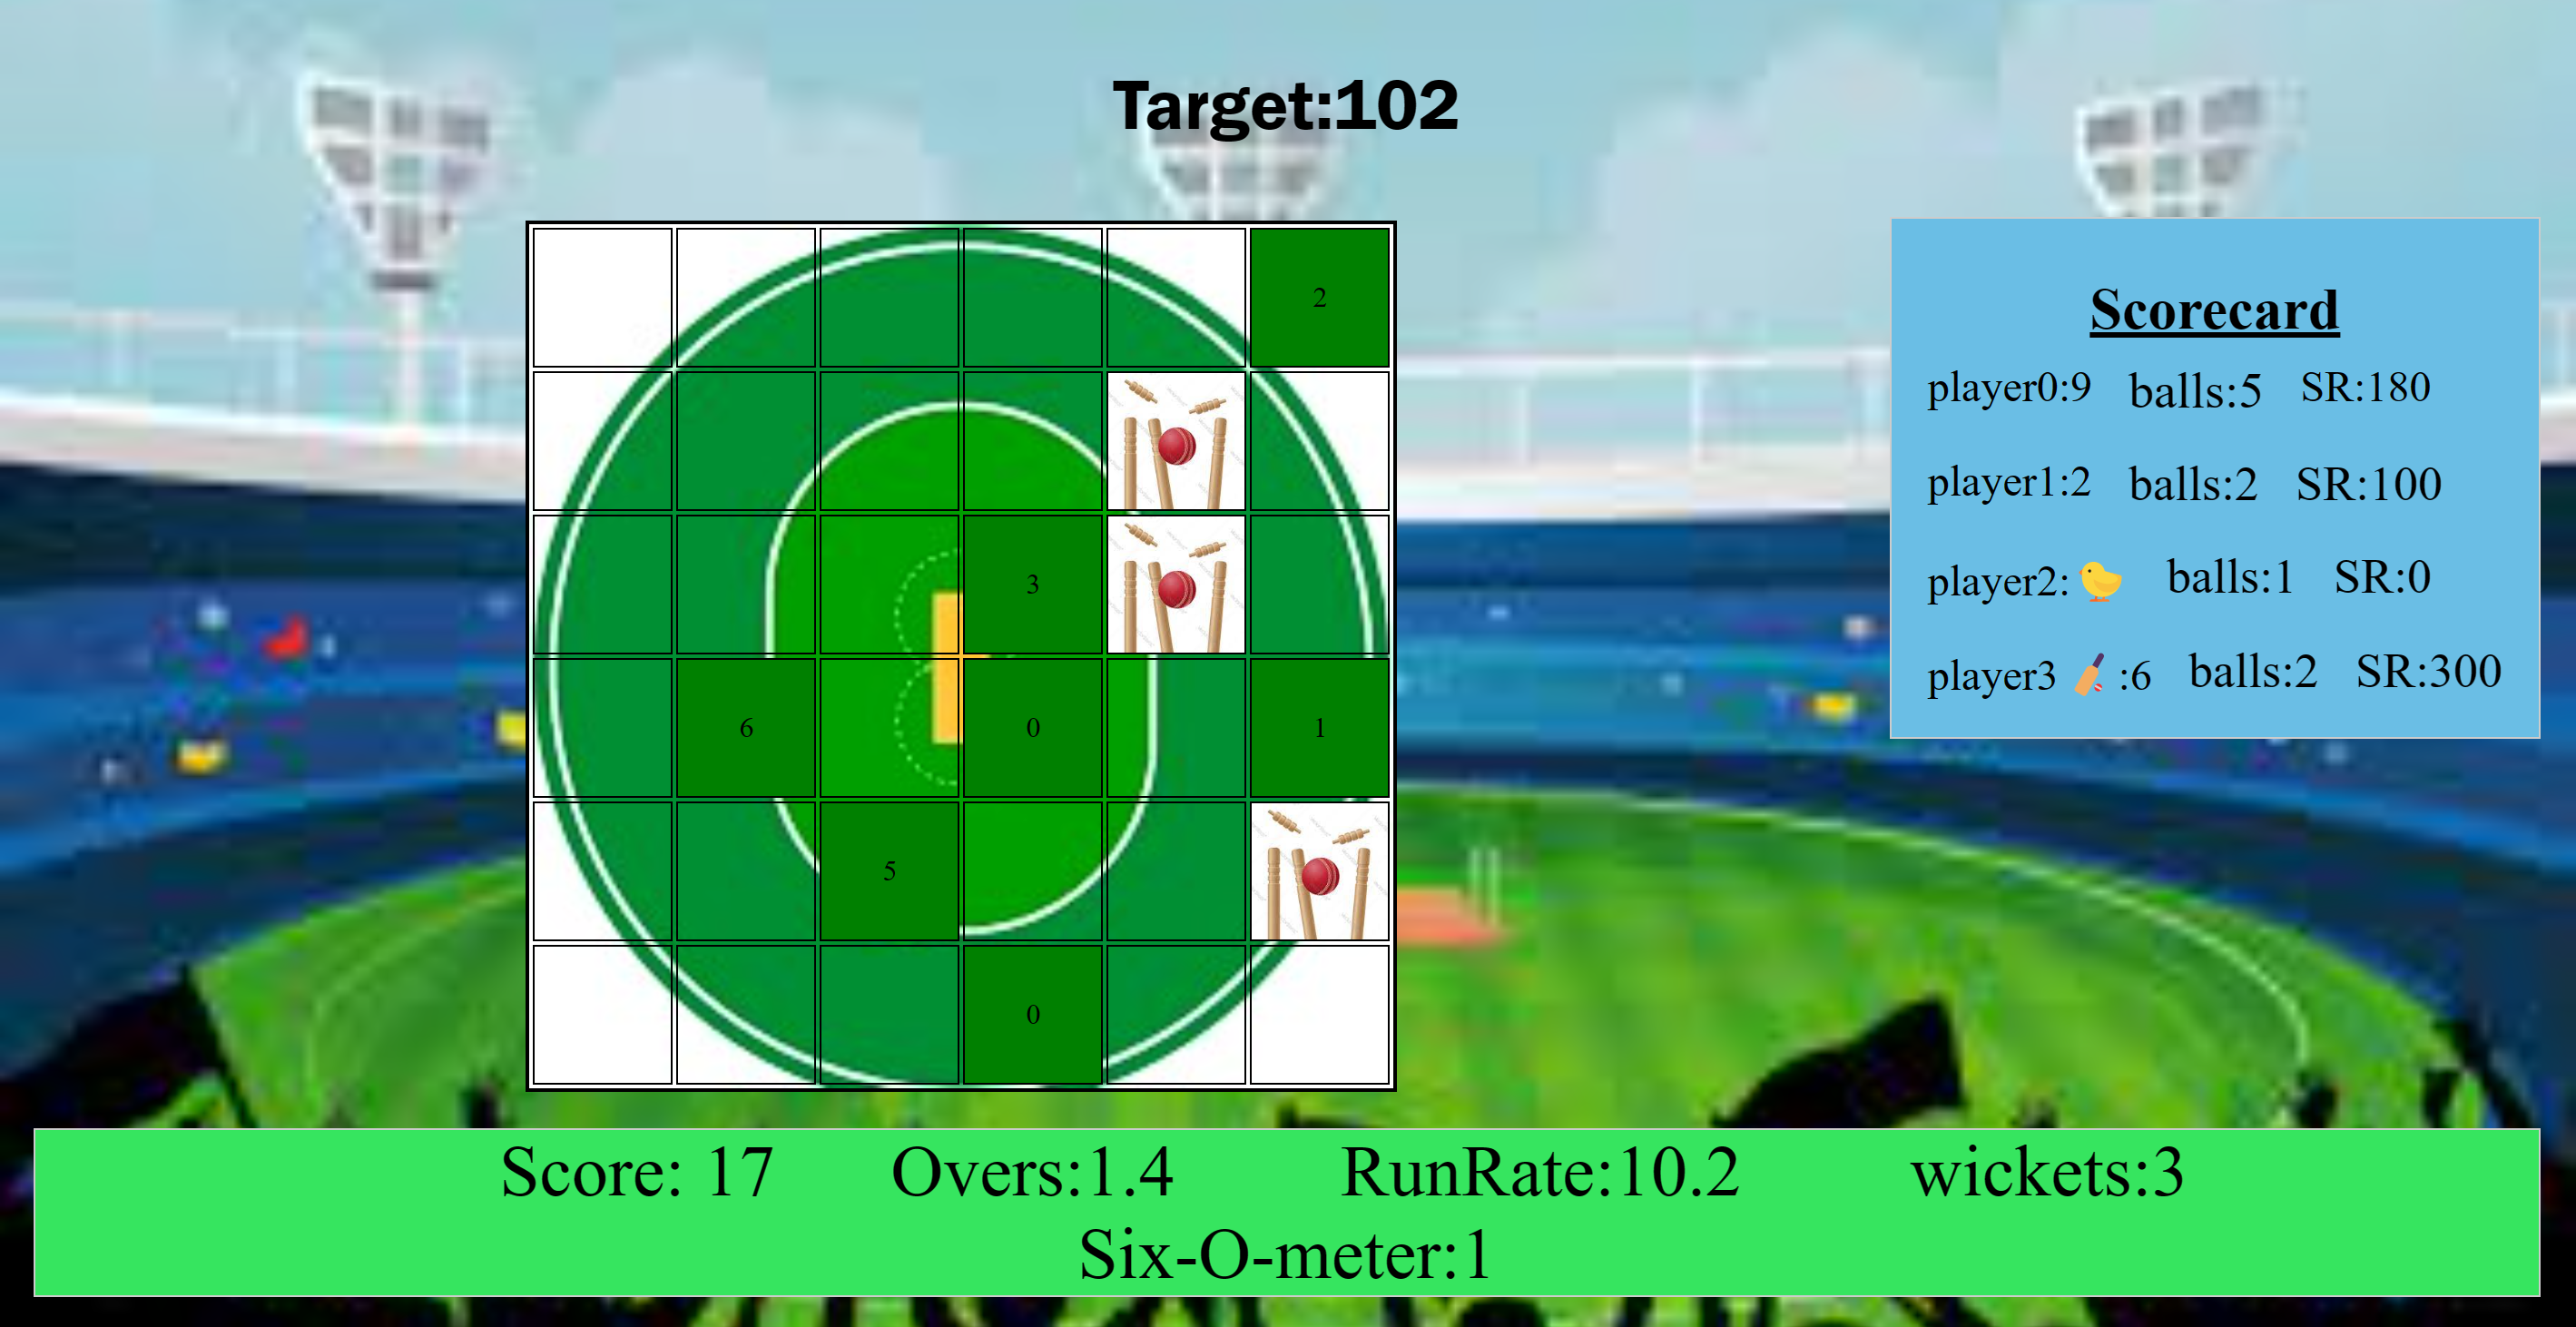
\includegraphics[width=1\textwidth]{inbetweena5wicketgame.png}
    \caption{Whileplaying}
    \label{fig:enter-label}
\end{figure}
\begin{figure}[H]
    \centering
    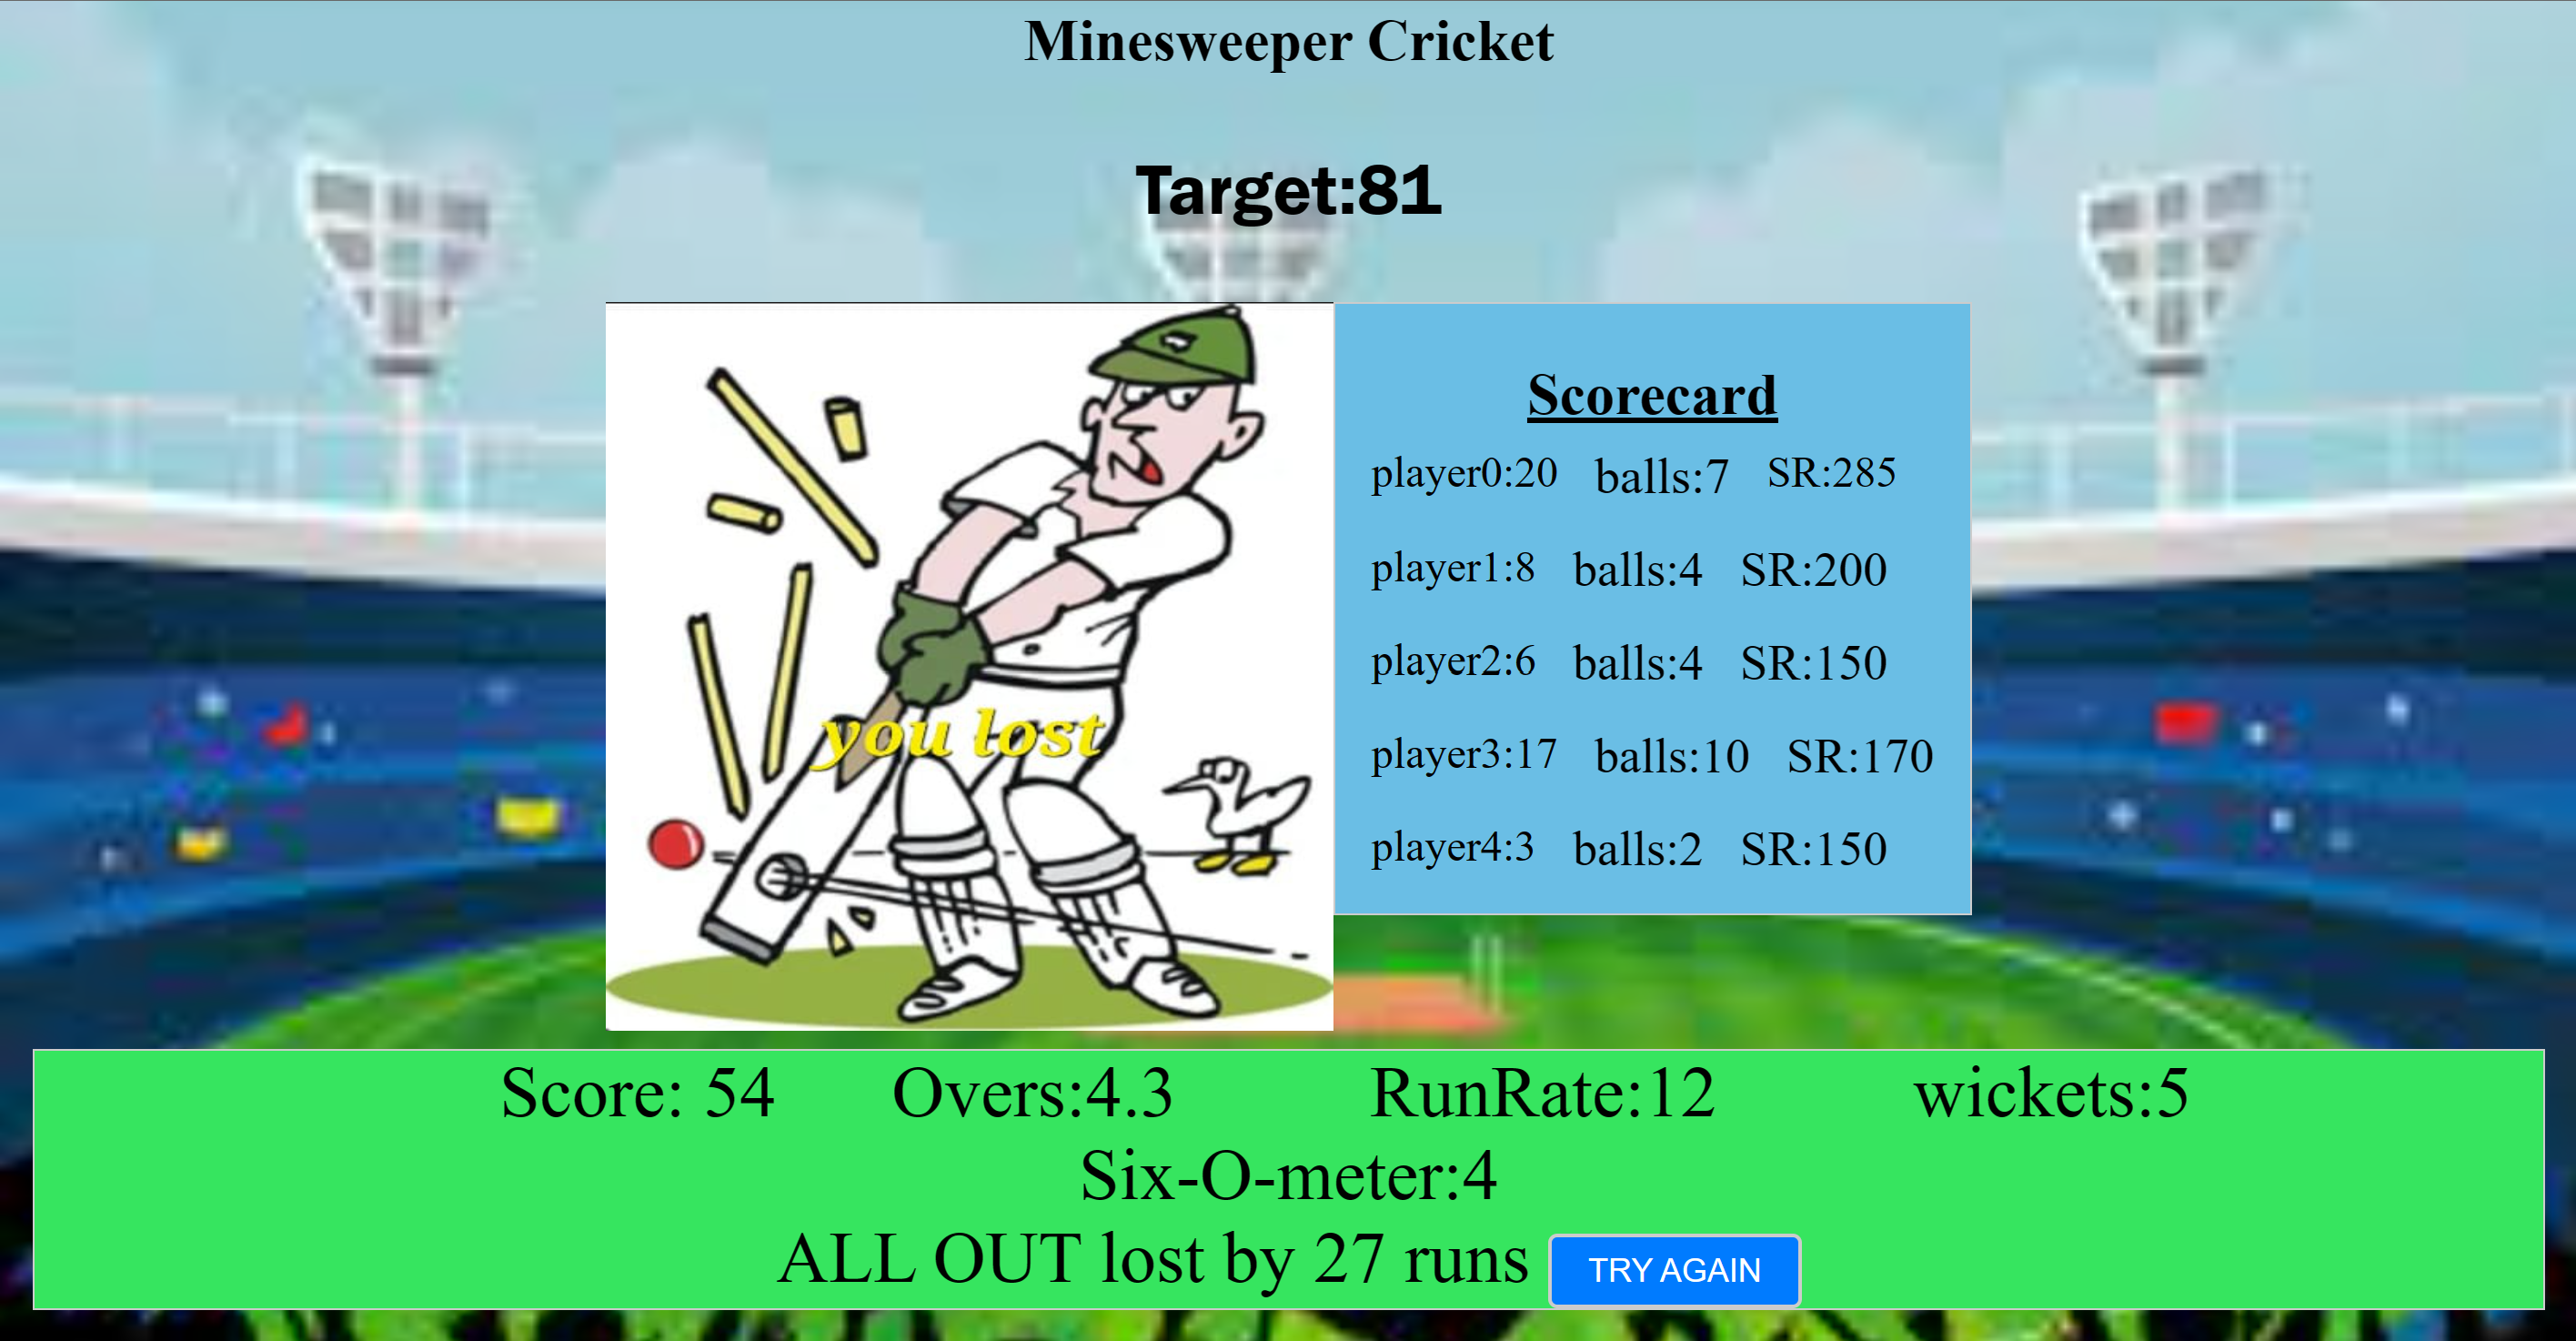
\includegraphics[width=1\textwidth]{Ifyoulose.png}
    \caption{If you lose}
    \label{fig:enter-label}
\end{figure}
\begin{figure}[H]
    \centering
    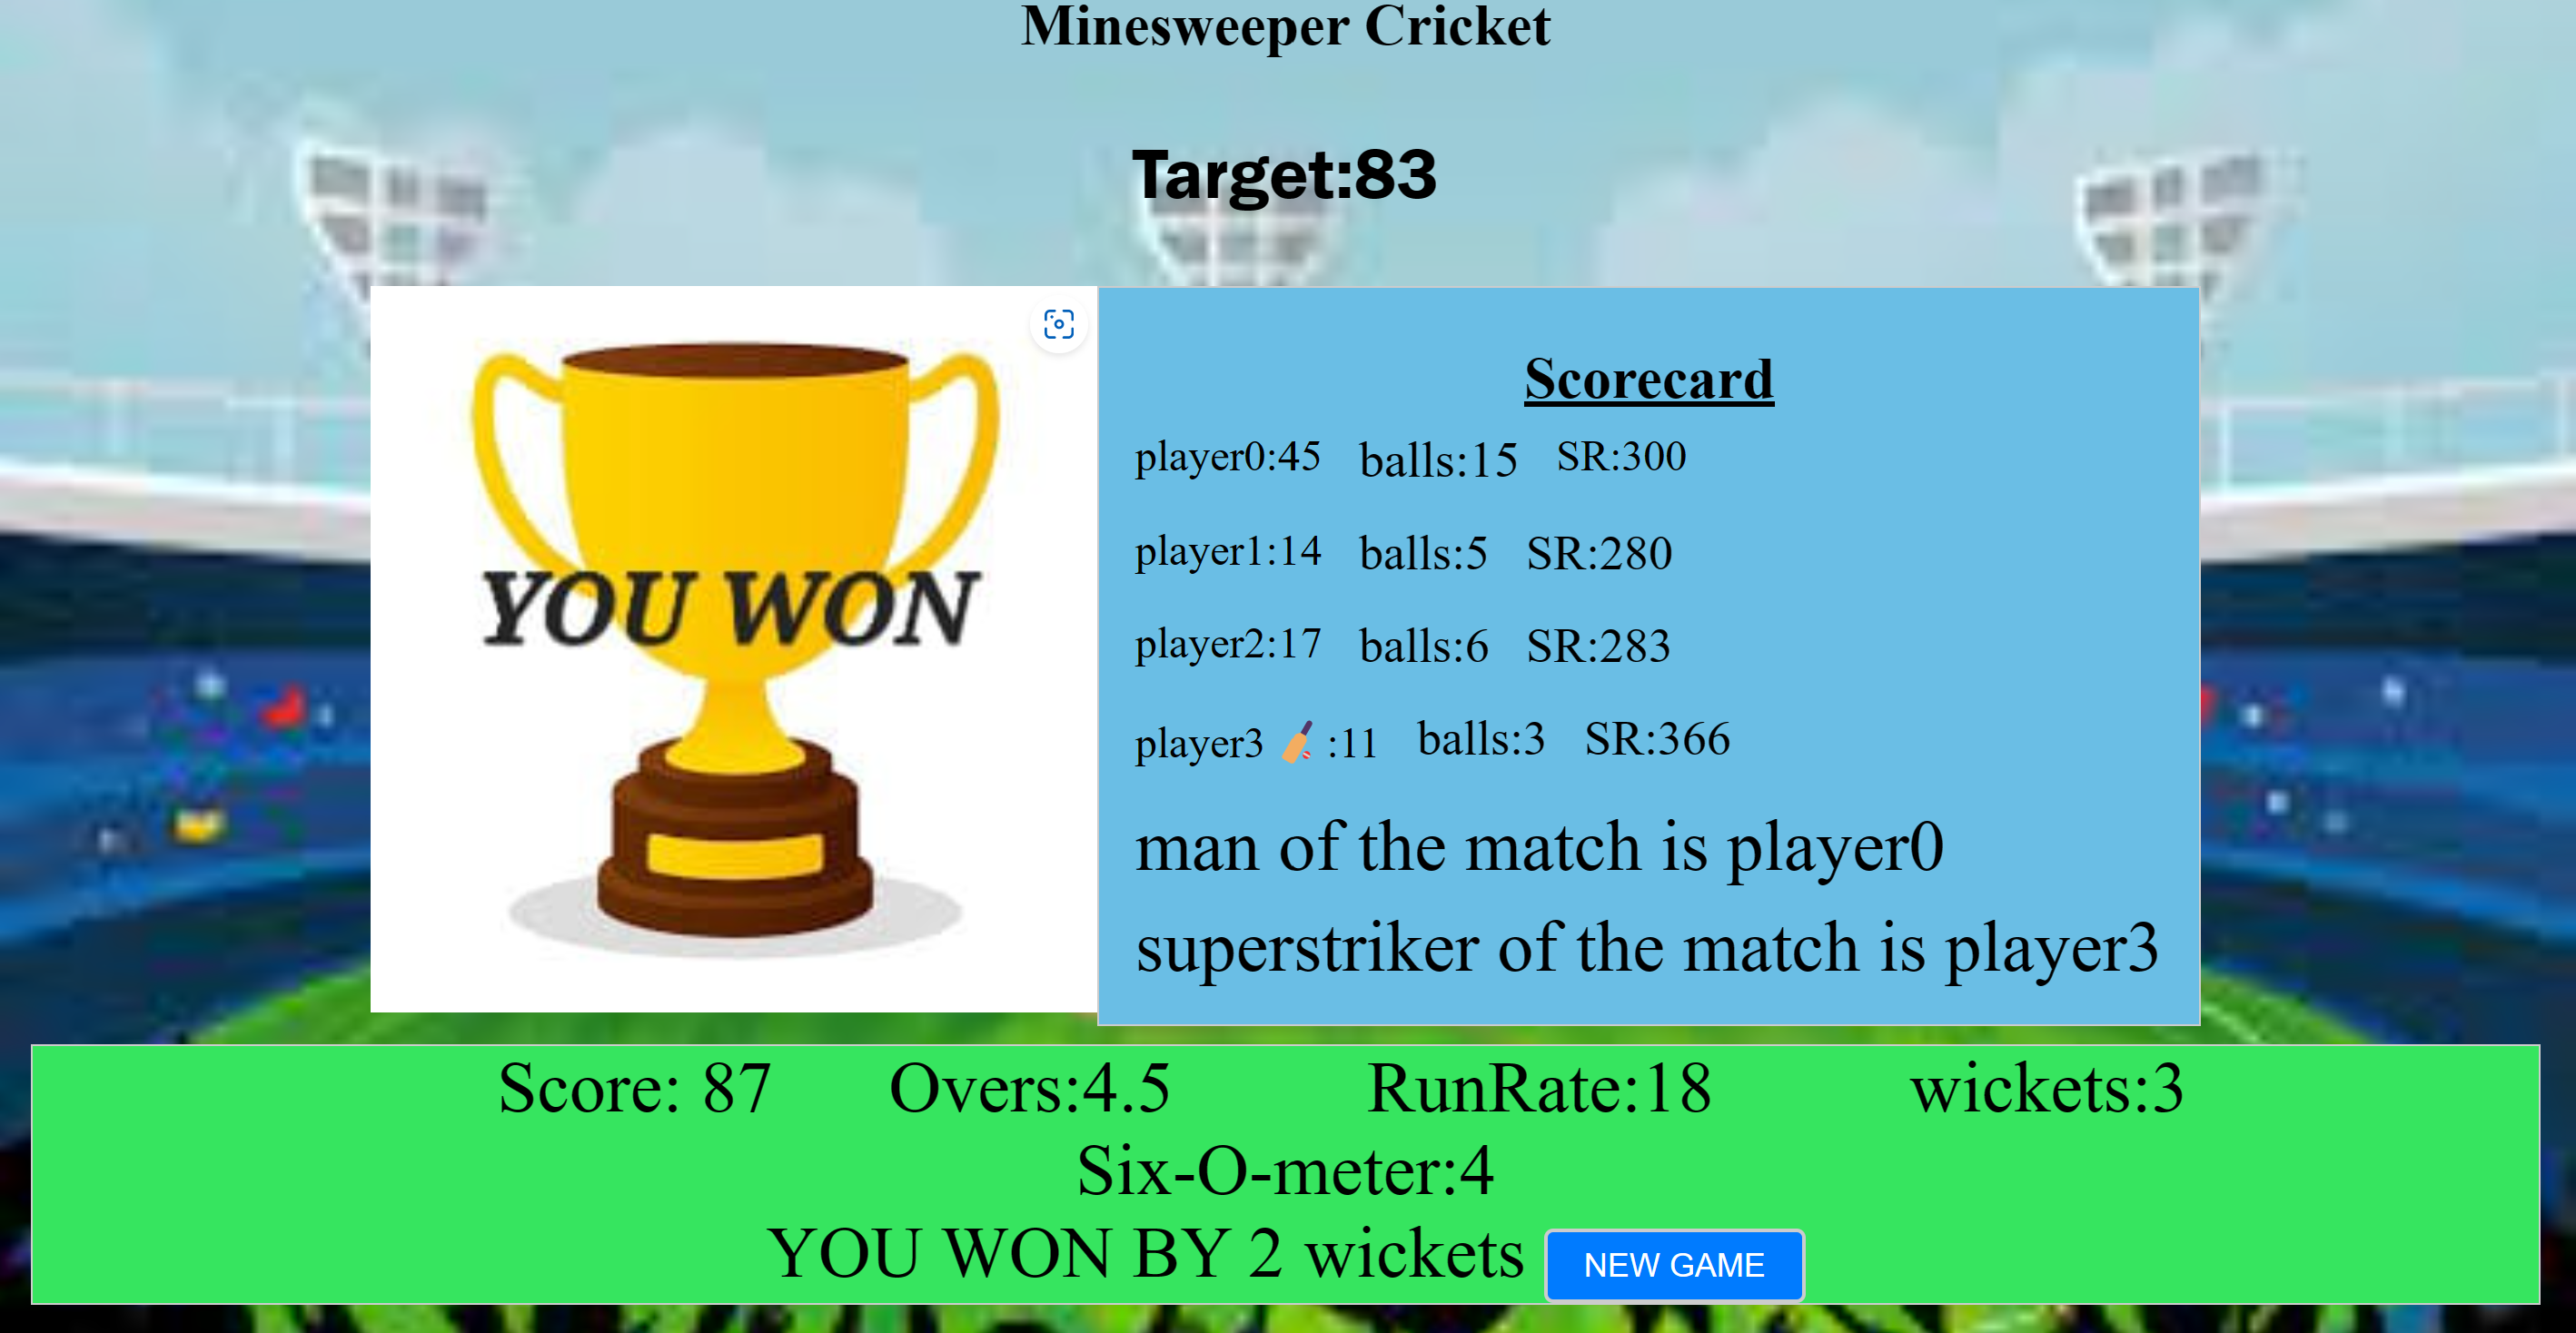
\includegraphics[width=1\textwidth]{ifyouwin.png}
    \caption{If you win}
    \label{fig:enter-label}
\end{figure}

\section{Resources}
Used this link to get basic idea about what minesweeper is nd copied the basic code required from it.
\href{https://iq.opengenus.org/minesweeper-game-using-js/}{minesweepergameusingjs}
for other parts I searched in internet for specific elements and how to implement


\end{document}
